\chapter{Estat de l'art}
\section{Aplicacions existents}
En quan a les aplicacions que es poden trobar actualment a \gls{Google_play}, la botiga virtual d'aplicacions per \gls{Android}, existeixen moltes que serveixen per a la gestió de despeses. És per això que s'estudiaran només les més rellevants i representatives, les quals tenen un mínim de 100.000 descarregues. Les aplicacions que s'han tingut en compte són les de la taula (\ref{fig:apps}). 

\begin{table}
\begin{tabular}{ | l | c | l | l | }
\hline
\headB{Núm.} & \headB{Icona} & \headB{Nom} & \headB{Autor} \\
\hline
App 1 & 
\includegraphics[scale=0.05]{A01_icon.png} & \href{https://play.google.com/store/apps/details?id=com.expensemanager}{Expense Manager} & Bishinews \\

App 2 & 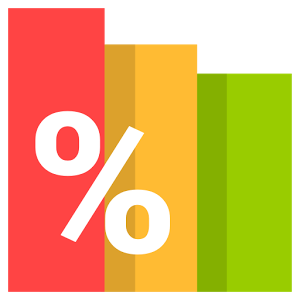
\includegraphics[scale=0.05]{A02_icon.png} & \href{https://play.google.com/store/apps/details?id=at.markushi.expensemanager}{Expense Manager} & Markus Hintersteiner \\

App 3 & 
\includegraphics[scale=0.05]{A03_icon.png} & \href{https://play.google.com/store/apps/details?id=com.bruno.myapps.droidwallet}{Droid Wallet} & William Bruno \\

App 4 & 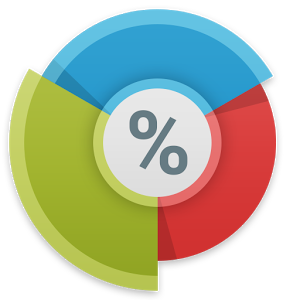
\includegraphics[scale=0.05]{A04_icon.png} & \href{https://play.google.com/store/apps/details?id=com.code44.finance}{Financius - Expense Manager} & Mantas Varnagiris \\

App 5 & 
\includegraphics[scale=0.05]{A05_icon.png} & \href{https://play.google.com/store/apps/details?id=com.handyapps.expenseiq}{Expense IQ} & Handy Apps \\

App 6 & 
\includegraphics[scale=0.05]{A06_icon.png} & \href{https://play.google.com/store/apps/details?id=com.techahead.ExpenseManager}{Diario Gasto Gerente (Daily Expense Manager)} & Gullak \\

App 7 & 
\includegraphics[scale=0.05]{A07_icon.png} & \href{https://play.google.com/store/apps/details?id=com.bookmark.money}{Money lover - Expense Manager} & ZooStudio   \\

App 8 & 
\includegraphics[scale=0.05]{A08_icon.png} & \href{https://play.google.com/store/apps/details?id=com.kpmoney.android}{AndroMoney (Expense Track)} & AndroMoney \\

App 9 & 
\includegraphics[scale=0.05]{A10_icon.png} & \href{https://play.google.com/store/apps/details?id=cz.destil.settleup}{Settle up} & David Vávra \\

App 10 & 
\includegraphics[scale=0.05]{A11_icon.png} & \href{https://play.google.com/store/apps/details?id=com.Splitwise.SplitwiseMobile}{Splitwise} & Splitwise \\

\hline
\end{tabular} 
\caption{Taula amb les aplicacions existents}
\label{fig:apps}
\end{table}

Actualment hi ha dos tipus d'aplicacions relacionades amb la gestió de despeses. Per una banda les que serveixen per enregistrar les despeses i/o ingressos personals, tot categoritzant-los (Aplicacions 1 - 8) i per l'altra les que serveixen per a gestionar despeses compartides en grup i/o deutes personals amb coneguts (Aplicacions 9 i 10).

%TODO More info about SUS. 
Per a veure el grau de satisfacció dels usuaris amb les aplicacions existents s'ha fet servir el qüestionari \gls{SUS} amb 4 usuaris. Amb els resultats s'ha fet la mitjana dels 4 usuaris per cada aplicació donant com a resultat els valors de la figura (\ref{fig:Apps_art_state}). Com es pot veure els usuaris no tenen una bona \ac{UX} al fer servir varies d'aquestes aplicacions, ja que obtenen una nota bastant baixa.

\begin{figure}[htp]
\centering
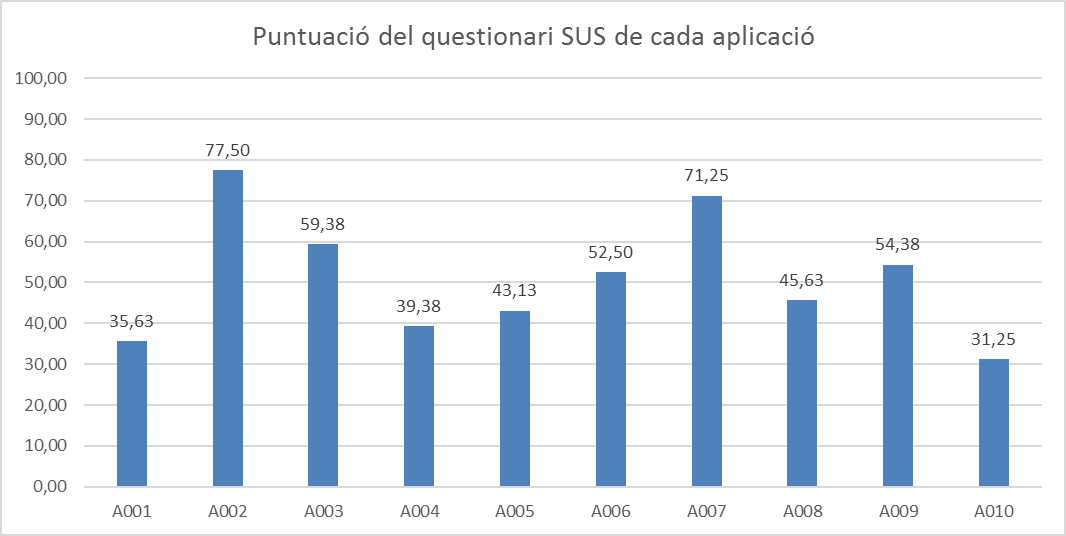
\includegraphics[scale=0.8]{Apps_art_state_SUS.png}
\caption{Puntuació de les aplicacions existents amb el questionari SUS}\label{fig:Apps_art_state}
\end{figure}

